\documentclass[a4paper,12pt]{article}

\usepackage[utf8]{inputenc}
\usepackage[margin=1.0in]{geometry}
\usepackage{graphicx}
\usepackage{mathtools}
\usepackage[table,xcdraw]{xcolor}

\title{Metaheuristic Training Neural Networks}

\date{April 20th, 2021}

\begin{document}

\maketitle

\begin{abstract}
This paper explores the use of metaheuristics in training a feed-forward artificial neural network, examining each algorithm and their performances in training a neural network versus backpropagation. Results show promise for the use of certain metaheuristics although the go-to approach of backpropagation is still superior in many ways.
\end{abstract}

\section{Introduction}



\section{Metaheuristics}

Metaheuristics are a type of "informed" local-global search which aim to optimize an objective function \cite{mh}. If the search space of a problem is known, it may be an appropriate scenario where a metaheuristic can optimize this problem. These algorithms are often accompanied by or designed with a metaphor in mind, which has lead to controversy \cite{crit}.



\subsection{Genetic Algorithm}

Genetic algorithm (\textbf{GA}) takes cues from evolutionary biology to evolve solutions to a problem based on both population and individual agent traits \cite{ga}.

\subsection{Particle Swarm Optimization}

Particle swarm optimization (\textbf{PSO}) is inspired by the flocking psychology of birds or other swarming animals \cite{pso}. 

\subsection{Differential Evolution}

Not too dissimilar to GA, differential evolution (\textbf{DE}) is another evolution-based metaheuristic but instead of inspired by biology, evolves solutions based on arithmetic and combining solutions according to some mathematical rules \cite{de}.

For DE, a population of solutions is generated randomly and are moved through the search space using arithmetic rules which allow combination of solutions. DE uses two parameters: \textit{crossover rate}, which determines the frequency in which solutions are combined, and \textit{differential weight}, which is a multiplicand determining how much of the difference between two crossovered solutions is imparted to the new solution.

While GA considers two parent chromosomes to generate two child chromosomes, DE contrastingly considers three "parent" solutions, combined in some ratio, to form a single new "child" solution. DE does not offer similar selection strategies like elitism as in GA, and instead a new population is guaranteed to be unique between generations.

Solutions evolve like so: for every solution $x$ in the population, three other solutions are chosen, $a, b, c$ such that $x, a, b, c$ are distinct entities from each other. A solution $y$ is generated according to the below:

\[
  y_i =
  \begin{cases}
    a_i + F \times (b_i - c_i) & \text{if $r_i < CR$ or $i = R$} \\
    x_i & \text{otherwise} \\
  \end{cases}
\]

$y$ is generated in sequence of axes $i = 1, 2, \dots, n$. For every solution that is created this way, a random index $R \in \{1, 2, \dots, n\}$ is chosen which signifies an axis which is always updated, even if crossover is not to occur. For this equation, $CR$ is the crossover rate and $F$ is the differential weight.

Once $y$ is found, it is compared to $x$, and if it has a better fitness, then $x$ is replaced with $y$ in the population and the process continues for other agents.

This type of evolution is not strictly bio-inspired and instead is more mathematical in nature. Crossover for DE allows the metaheuristic to have an \textit{exploratory factor}, where the search space is explored in larger steps when compared to an \textit{exploitative factor}, where solutions are fine-tuned in place to reach optima around the current solution position. DE still exhibits an exploitative factor, as when the population converges to an optima, all solutions within the population more closer resemble each other, meaning exploration is minute.

Over time, the best fitness of solutions in the population is improved until convergence (either to a global optimum or local optima). Every generation is assured to either remain the same or improve since a fitness comparison is the criteria for a solution being replaced. In other words, solutions will never regress to a worse solution.

\subsection{Bat Algorithm}

Bat algorithm (\textbf{BA}) is similar to other metaheuristics in that it is a swarm-based approach to improving solutions. Solutions within the search space are updated similar to how swarming microbats descend onto prey or food \cite{ba}.

\section{Network Training}

A neural network is bio-inspired tool under the broader class of machine learning algorithms. It consists of a sequence of layers, themselves containing nodes---called neurons. The biology analogy is the brain, where this technique of machine learning takes its namesake  \cite{mitchell}. Neural networks can be used for many tasks, although the classical usage is one of classification: using a neural network to train a model which can be used as a classifier.

The layers between neural network layers are composed of synaptic weights: these weights are mathematical links between neurons and signify how strong a signal between neurons is. In the simplest sense, a synaptic weight is some multiplicand between neurons, altering the signal between them.

One of the most popular approaches to training a neural network is using \textit{backpropagation} (\textbf{BP}), which is a gradient-based training mechanism which relies on the existence of an error gradient between a target output value and the actual found output value. 

Training patterns are inputted into the network at the first layer, travel to subsequent layers through a \textit{feedforward} process, then when in the output layer, the error is calculated as a function of target and actual values. The error signal is backpropagated through the network in reverse, adjusting the synaptic weights as needed so the model more closely resembles the training pattern.

Given enough training patterns and enough iterations or repetitions of the process, ultimately---and provided appropriate network parameters are chosen---the network model is able to classify not only previous data fed into it, but also novel data from the same data set.

However, BP is mathematically robust yet conceptually obtuse: oftentimes neural networks are referred as black-boxes, as while the inputs and outputs are known, the inner workings are abstract. Thus while BP is an adequate training mechanism for a neural network, alternatives exist such as the use of metaheuristics.

\begin{figure}[h!]
\centering

\includegraphics[scale=0.65]{images/weight-visualization.png}
\caption{Connections between layers can be enumerated as a set of weights.}
\label{fig:weight-vis}
\end{figure}

In the previous figure, a simple 2-1-2 network is shown and each synaptic weight connecting each layer is enumerated. For this network, which presents a 4-dimensional problem space, it has four weights.

Since metaheuristics explore the search space, it's useful to think of solutions as a position in $n$-space, where $n$ is the dimensionality of the problem. For this example network, solutions update themselves in a 4-dimensional search space.

Each metaheuristic tested either takes literal sense of this concept---bat algorithm having bat agents with a specific position, as example---or are more abstract or have no close conceptual similarity to an agent "moving". Nevertheless, they all function in an identical fashion.

Since synaptic weights are enumerable in this way, it is simple to decode the network as instead a position in $n$-space. For this reason, a network can be be represented as a solution for a metaheuristic.

To use an example, a GA chromosome can be created as some encoding of the network synaptic weights. A network of weights $[w_0, w_1, ..., w_n]$ can be encoded as a chromosome of genes $[x_0, x_1, ..., x_n]$, where $x_i = w_i$. Likewise, this encoding is reversible, where for this sample a chromosome can be translated into a network.

This translation is integral to the inter-connectivity between a network and its metaheuristic training mechanism, as a metaheuristic cannot be perform on a network directly.

\begin{figure}[h!]
\centering
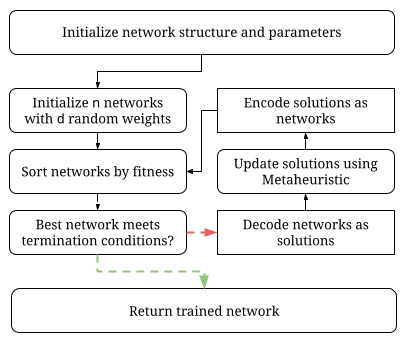
\includegraphics[scale=0.75]{images/training-visualization.png}
\caption{Metaheuristic adapted for training a neural network.}
\label{fig:training-vis}
\end{figure}

In the previous figure it is shown how a metaheuristic is integrated within a neural network's training process. For this figure, $d$ is the dimensionality of the network---how many synaptic weights exist in the network---and $n$ is the number of agents for use with the metaheuristic.

Since metaheuristics are population based, this method of training neural networks is analogous to training laterally multiple networks at once and using both the traits of the population and individual solutions to improve.

\section{Experimental Setup}

To evaluate the efficacy of metaheuristics in training a neural network, a standard feedforward network was implemented alongside implementation of each training mechanism: backpropagation (\textbf{BP-NN}), genetic algorithm (\textbf{GA-NN}), particle swarm optimization (\textbf{PSO-NN}), differential evolution (\textbf{DE-NN}), and bat algorithm (\textbf{BA-NN}).

Further, a testing suite was devised to train a model using each training mechanism and collect the results in the form of error over time curves. The error function used is mean squared error (\textbf{MSE}).

This suite performs each training 100 times for each data set and then discards the worst 20\% of runs, as the mean of runs should be indicative of generally good results. A poor training attempt would normally be discarded and here is no different. Runs are then aggregated and the mean is found to be plotted.

Training ceases when one of two conditions are met: either the MSE of the network has reached a value of $0.1$ or below, or the maximum number of epochs has elapsed. In the case where convergence did not occur without the defined number of epochs, that training technique is determined to have not converged.

Consideration has to be given for network and training parameters which vary by data set. Additionally, the data sets themselves need to be examined.

\subsection{Data}

Six data sets were used: \textit{Iris} \cite{data} for classification of species of iris flowers, \textit{Penguins} \cite{penguins} for classification of penguin species, \textit{Wheat Seeds} \cite{data} for classification of wheat varieties, \textit{Wine} \cite{data} for classification of wine varieties, \textit{Breast Cancer} \cite{data} for classification of breast cancer diagnosis, and \textit{Ionosphere Radar} \cite{data}. These data sets were chosen as they increase in complexity at a generally consistent rate, allowing for scalability of metaheuristic training to be considered.

Rows in the data set comprise of input patterns which are separated into attributes---of which there are many---and classifications---of which there is one, albeit with multiple possible values. The network structured initialized for a given data set is a consequence of these variables: the input layer contains a number of neurons equal to the number of attributes of the data, and the output layer contains a number of neurons equal to the number of distinct possible classifications of the data.

\begin{table}[h!]
\centering
\begin{tabular}{|c|c|c|c|}
\hline
\textbf{Data Set} & \textbf{Instances} & \textbf{Attributes} & \textbf{Classes} \\ \hline
\textit{Iris} & 151 & 4 & 3 \\ \hline
\textit{Penguins} & 333 & 6 & 3 \\ \hline
\textit{Wheat Seeds} & 211 & 7 & 3 \\ \hline
\textit{Wine} & 178 & 13 & 3 \\ \hline
\textit{Breast Cancer} & 570 & 31 & 2 \\ \hline
\textit{Ionosphere Radar} & 352 & 34 & 2 \\ \hline
\end{tabular}
\caption{Data sets used for results collection.}
\label{Tab:data-sets}
\end{table}

In the previous table, this information is tabulated. While the input and output layers of the network is decided by the data, the hidden layer size is arbitrary but still chosen through some experimentation. A smaller hidden layer will train faster, but too small will result in poor results. Experimentation was performed to minimize the hidden layer size while still maintaining satisfactory results.

\begin{table}[h!]
\centering
\begin{tabular}{|c|c|c|c|c|}
\hline
\textbf{Data Set} & \textbf{IL Size} & \textbf{HL Size} & \textbf{OL Size} & \textbf{Dimensionality} \\ \hline
\textit{Iris} & 4 & 3 & 3 & 27 \\ \hline
\textit{Penguins} & 6 & 4 & 3 & 43 \\ \hline
\textit{Wheat Seeds} & 7 & 5 & 3 & 58 \\ \hline
\textit{Wine} & 13 & 6 & 3 & 105 \\ \hline
\textit{Breast Cancer} & 31 & 8 & 2 & 274 \\ \hline
\textit{Ionosphere Radar} & 34 & 10 & 2 & 372 \\ \hline
\end{tabular}
\caption{Dimensionality of each problem.}
\label{Tab:dim-tab}
\end{table}

In the previous table, the dimensionality of each classification problem is found as a function of network topology. Declaratively, the dimensionality of a network problem is found using the below equation:

$$d = (HL \times (IL + 1)) + (OL \times (HL + 1))$$

Dimensionality is related to how "difficult" the classification problem is: while data can be intrinsically complex, dimensionality gives a general idea of how complicated it will be to train a network using that data.

\subsection{Parameters}

Each network is initialized with a few parameters, some of which are specific to each metaheuristic used. Many oarameters remain consistent between training methods, but many parameters are initialized on a per-problem basis.

All parameters are chosen through some trial-and-error as there are often no "one size fits all" approach to parameter selection and tuning. Parameters chosen provide generally good results but could be improved, perhaps by an optimization algorithm.

\subsubsection{Consistent Parameters}

Parameters related to network topology and the training process are consistent between data sets and metaheuristics. Three parameters, the number of epochs, the holdout ratio, and the initial weight range are fixed for all problems.

\begin{table}[h!]
\centering
\begin{tabular}{|c|c|c|}
\hline
\textbf{Epochs} & \textbf{Holdout Ratio} & \textbf{Initial Weight Range} \\ \hline
100 & 0.70 & {[}-0.50, 0.50{]} \\ \hline
\end{tabular}
\caption{Constant network parameters.}
\label{Tab:const-par}
\end{table}

In the previous table, the three constant network parameters are tabulated. Epochs is the amount of training iterations performed and is one of the termination conditions for training, the holdout ratio is the proportion of input data to be used for training the network versus testing the network, and the initial weight range is the range between minimum and maximum values for weight initialization.

Since this is a comparative study between BP and metaheuristics, BP as the default decides many of these parameters. For example, for a metaheuristic to be relatively viable, the number of epochs should not be too dissimilar for metaheuristics: to this end, 100 epochs was chosen as BP could train within this amount in every scenario. The same applies for the other two parameters.

Likewise, hidden layer size is a constant, but only between training methods: this parameter varies only by data set used.

\begin{table}[h!]
\centering
\begin{tabular}{|c|c|}
\hline
\textbf{Data Set} & \textbf{Hidden Layer Size} \\ \hline
\textit{Iris} & 3 \\ \hline
Penguins & 4 \\ \hline
Wheat Seeds & 5 \\ \hline
Wine & 6 \\ \hline
Breast Cancer & 8 \\ \hline
Ionosphere Radar & 10 \\ \hline
\end{tabular}
\caption{Hidden layer size per data set.}
\label{Tab:hl-tab}
\end{table}

In the previous table, the hidden layer size is tabulated per data set. Since the difference between BP and metaheuristics is being examined, this needs to remain equal as all training methods are effectively training identical networks.

\subsubsection{BP-NN}

BP relies on two parameters: \textit{learning rate}, or the amount of correction a synaptic weight should take from the training instance, and \textit{momentum rate}, which considers some portion of the prior training instance when updating using the current training instance.

\begin{table}[h!]
\centering
\begin{tabular}{|c|c|c|}
\hline
\textbf{Data Set} & \textbf{LR} & \textbf{MR} \\ \hline
\textit{Iris} & 0.100 & 0.001 \\ \hline
\textit{Penguins} & 0.100 & 0.001 \\ \hline
\textit{Wheat Seeds} & 0.100 & 0.001 \\ \hline
\textit{Wine} & 0.100 & 0.002 \\ \hline
\textit{Breast Cancer} & 0.100 & 0.003 \\ \hline
\textit{Ionosphere Radar} & 0.100 & 0.002 \\ \hline
\end{tabular}
\caption{Backpropagation parameters.}
\label{Tab:bp-par}
\end{table}

In the previous table, BP-NN parameters are tabulated per data set, where $LR$, $MR$ are learning rate and momentum rate respectively.

Since BP is a single-agent training mechanism, it does not have a population as metaheuristics do.

\subsubsection{GA-NN}

For the first metaheuristic, GA considers six parameters for training. They are the population size (how many chromosomes), crossover rate, mutation rate, elite proportion, tournament proportion, and a base mutation value.

\begin{table}[h!]
\centering
\begin{tabular}{|c|c|c|c|c|c|c|}
\hline
\textbf{Data Set} & \textbf{Population} & \textbf{CR} & \textbf{MR} & \textbf{$E_p$} & \textbf{$T_p$} & \textbf{Base} \\ \hline
\textit{Iris} & 100 & 0.90 & 0.03 & 0.05 & 0.03 & 0.5 \\ \hline
\textit{Penguins} & 100 & 0.90 & 0.03 & 0.05 & 0.03 & 0.5 \\ \hline
\textit{Wheat Seeds} & 100 & 0.90 & 0.04 & 0.05 & 0.04 & 0.6 \\ \hline
\textit{Wine} & 100 & 0.90 & 0.05 & 0.05 & 0.05 & 0.7 \\ \hline
\textit{Breast Cancer} & 100 & 0.90 & 0.05 & 0.05 & 0.07 & 0.8 \\ \hline
\textit{Ionosphere Radar} & 100 & 0.90 & 0.06 & 0.05 & 0.09 & 0.9 \\ \hline
\end{tabular}
\caption{Genetic algorithm parameters.}
\label{Tab:ga-par}
\end{table}

In the previous table, GA-NN parameters are tabulated per data set, where $CR$, $MR$, $E_p$, $T_p$ are the crossover rates, mutation rates, elite proportions, and tournament proportions respectively.

\subsubsection{PSO-NN}

PSO has five different parameters controlling its movement: population size, inertial weight, cognitive and social coefficients, and a boundary variable.

\begin{table}[h!]
\centering
\begin{tabular}{|c|c|c|c|c|c|}
\hline
\textbf{Data Set} & \textbf{Population} & \textbf{$\omega$} & \textbf{$c_1$} & \textbf{$c_2$} & \textbf{Boundary} \\ \hline
\textit{Iris} & 100 & 0.5 & 1.5 & 1.2 & 3 \\ \hline
\textit{Penguins} & 100 & 0.5 & 1.4 & 1.3 & 4 \\ \hline
\textit{Wheat Seeds} & 100 & 0.6 & 1.3 & 1.1 & 5 \\ \hline
\textit{Wine} & 100 & 0.3 & 1.6 & 1.4 & 7 \\ \hline
\textit{Breast Cancer} & 100 & 0.4 & 1.4 & 1.1 & 7 \\ \hline
\textit{Ionosphere Radar} & 100 & 0.3 & 1.3 & 1.3 & 9 \\ \hline
\end{tabular}
\caption{Particle swarm optimization parameters.}
\label{Tab:pso-par}
\end{table}

In the previous table, these parameters are tabulated per data set, where $\omega$ is the inertial weight and $c_1$, $c_2$ are the cognitive and social coefficients respectively.

\subsubsection{DE-NN}

DE only has three parameters: population size, crossover rate, and differential weight.

\begin{table}[h!]
\centering
\begin{tabular}{|c|c|c|c|}
\hline
\textbf{Data Set} & \textbf{Population} & \textbf{CR} & \textbf{F} \\ \hline
\textit{Iris} & 50 & 0.90 & 0.25 \\ \hline
\textit{Penguins} & 50 & 0.90 & 0.35 \\ \hline
\textit{Wheat Seeds} & 50 & 0.90 & 0.25 \\ \hline
\textit{Wine} & 50 & 0.90 & 0.20 \\ \hline
\textit{Breast Cancer} & 50 & 0.90 & 0.15 \\ \hline
\textit{Ionosphere Radar} & 50 & 0.90 & 0.10 \\ \hline
\end{tabular}
\caption{Differential evolution parameters.}
\label{Tab:de-par}
\end{table}

Above are the DE-NN parameters tabulated, where $CR$ is the crossover rate and $F$ is the differential weight.

\subsubsection{BA-NN}

Lastly, BA has six parameters: population size, frequency minimum and maximum, a boundary, a loudness decreasing factor, and a pulse rate increasing factor.

\begin{table}[h!]
\centering
\begin{tabular}{|c|c|c|c|c|c|c|}
\hline
\textbf{Data Set} & \textbf{Population} & \textbf{$F_{min}$} & \textbf{$F_{max}$} & \textbf{Boundary} & \textbf{$\alpha$} & \textbf{$\gamma$} \\ \hline
\textit{Iris} & 100 & 0 & 2 & 3 & 0.90 & 0.90 \\ \hline
\textit{Penguins} & 100 & 0 & 2 & 4 & 0.90 & 0.90 \\ \hline
\textit{Wheat Seeds} & 100 & 0 & 2 & 5 & 0.90 & 0.90 \\ \hline
\textit{Wine} & 100 & 0 & 2 & 7 & 0.90 & 0.90 \\ \hline
\textit{Breast Cancer} & 100 & 0 & 2 & 7 & 0.90 & 0.90 \\ \hline
\textit{Ionosphere Radar} & 100 & 0 & 2 & 9 & 0.90 & 0.90 \\ \hline
\end{tabular}
\caption{Bat algorithm parameters.}
\label{Tab:ba-par}
\end{table}

Here tabulated, the BA-NN parameters $F_{min}$, $F_{max}$ are the frequency minimum and maximum values and $\alpha$, $\gamma$ are the loudness decreasing factor and pulse rate increasing factor respectively.

\section{Experimental Results}

Every network is trained according to the previously defined test structures. Plots are then generated allowing a visual aid to compare. Two statistical tests are also performed on the data: an ANOVA test and Tukey's HSD test.

The ANOVA test is designed to determine if multiple samples come from the same population; in other words, the ANOVA test is used for testing purposes to identify if all training techniques are the same or there is non-trivial differences between them. An ANOVA test produces two statistics that are relevant: an $F$-score, where an $F >= 1.0$ denotes confidence in the test, and a $p$-value, where a $p <0.05$ suggests there is significance in choosing some training techniques over the others.

Tukey's HSD test, if an ANOVA test shows significance, will then identify where outliers exist by doing pairwise comparison of means and variances between samples. If better training methods exist, they will become evident more directly using this test.

Plots show a curve for each training method, where each curve is the MSE over time. At the bottom of each plot is a tickmark which denotes at what epoch, on average, the training method reached a termination condition.

\pagebreak

\subsection{Iris}

Using the Iris data set and network parameters as defined previously for each training method, the below plot is found:

\begin{figure}[h!]
\centering
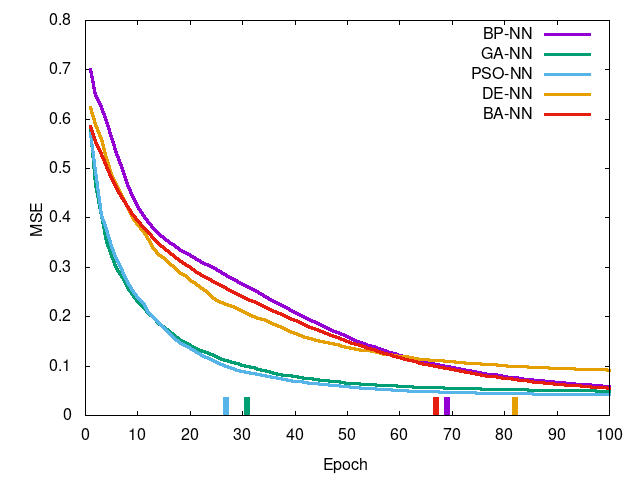
\includegraphics[scale=0.65]{images/iris-plot.png}
\caption{Iris test results for metaheuristics and backpropagation.}
\label{fig:iris}
\end{figure}

Visually, two training techniques (PSO-NN and GA-NN) converged to a termination condition much faster than the other three.

To determine if this difference is of statistic importance, an ANOVA test is run using each curve as a sample. This test yields an $F = 17.65$ and a $p < 0.001$ which suggests there is high confidence that there are some training methods that outperform the others.

Tukey's HSD test is then performed showing no significance between GA-NN and PSO-NN. Likewise it shows no significance between BP-NN, DE-NN, and BA-NN. However, samples between each grouping does show significance.

Since Tukey's HSD test showed significance between two groups, on comparing the mean number of epochs it took to reach termination condition, it can be concluded that GA-NN and PSO-NN outperform the other training methods and to a largely significant degree.

\begin{table}[h!]
\centering
\begin{tabular}{c|c|c|c|c|c|}
\cline{2-6}
 & \textbf{BP-NN} & \textbf{GA-NN} & \textbf{PSO-NN} & \textbf{DE-NN} & \textbf{BA-NN} \\ \hline
\multicolumn{1}{|c|}{\textit{Min}} & \cellcolor[HTML]{FFCCC9}51 & \cellcolor[HTML]{C5F1BF}9 & 10 & 36 & 31 \\ \hline
\multicolumn{1}{|c|}{\textit{Avg}} & 70 & 31 & \cellcolor[HTML]{C5F1BF}27 & \cellcolor[HTML]{FFCCC9}82 & 67 \\ \hline
\end{tabular}
\caption{Minimum and average time to terminate for Iris data set.}
\label{Tab:iris-min}
\end{table}

Tabulated above is the minimum and mean number of epochs it took to reach a termination condition, green denoting best, and red worst. Here, BP-NN was the slowest network to converge, but on average, DE-NN was the slowest to converge. Agreeing with our results from before, both GA-NN and PSO-NN outperform the others significantly, having the fastest training at once and on average.

\pagebreak

\subsection{Penguins}

The Penguins data set is then trained upon using network parameters as defined previously for each training method, producing the below plot:

\begin{figure}[h!]
\centering
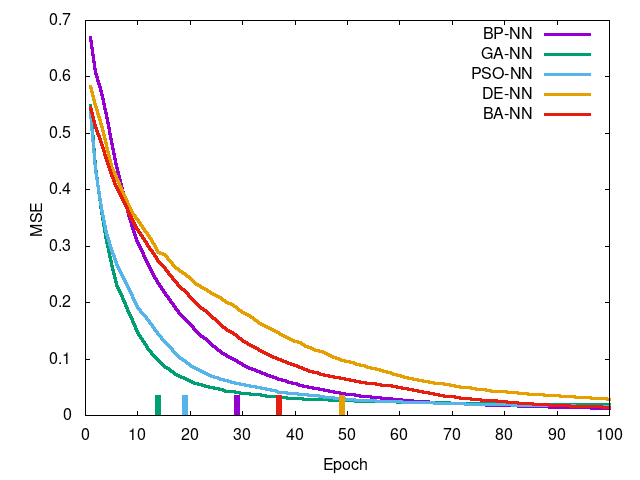
\includegraphics[scale=0.65]{images/penguins-plot.png}
\caption{Penguins test results for metaheuristics and backpropagation.}
\label{fig:penguins}
\end{figure}

It is difficult to discern visually whether curves come from the same distribution, so again an ANOVA test is performed. This test yields an $F = 9.0332$ and $p < 0.001$ which suggests there is confidence in curves not coming from the same population: outliers exist between training methods.

To identify them, Tukey's HSD test is performed, showing significance only between DE-NN and both GA-NN and PSO-NN. Here DE-NN is an outlier as the other samples show no significant difference.

From these tests, it is shown there is no significance in choosing between GA-NN, PSO-NN, BP-NN, or BA-NN; however, DE-NN is significantly slower than the other four.

\begin{table}[h!]
\centering
\begin{tabular}{c|c|c|c|c|c|}
\cline{2-6}
 & \textbf{BP-NN} & \textbf{GA-NN} & \textbf{PSO-NN} & \textbf{DE-NN} & \textbf{BA-NN} \\ \hline
\multicolumn{1}{|c|}{\textit{Min}} & \cellcolor[HTML]{FFFFFF}20 & \cellcolor[HTML]{FFFFFF}7 & \cellcolor[HTML]{C5F1BF}6 & \cellcolor[HTML]{FFCCC9}26 & \cellcolor[HTML]{FFFFFF}18 \\ \hline
\multicolumn{1}{|c|}{\textit{Avg}} & \cellcolor[HTML]{FFFFFF}29 & \cellcolor[HTML]{C5F1BF}14 & \cellcolor[HTML]{FFFFFF}19 & \cellcolor[HTML]{FFCCC9}49 & \cellcolor[HTML]{FFFFFF}37 \\ \hline
\end{tabular}
\caption{Minimum and average time to terminate for Penguins data set.}
\label{Tab:penguins-min}
\end{table}

In the previous table, as before the minimum and average number of epochs to reach a termination condition is given for each network type. As well, as before both GA-NN and PSO-NN are the fastest to train either as a single training or on average. DE-NN as found using the tests before was the slowest in every regard.

\pagebreak

\subsection{Wheat Seeds}

Then, the Wheat Seeds data set is trained upon to attempt to make a model at classifying the data. Using the defined network parameters, the below plot is found:

\begin{figure}[h!]
\centering
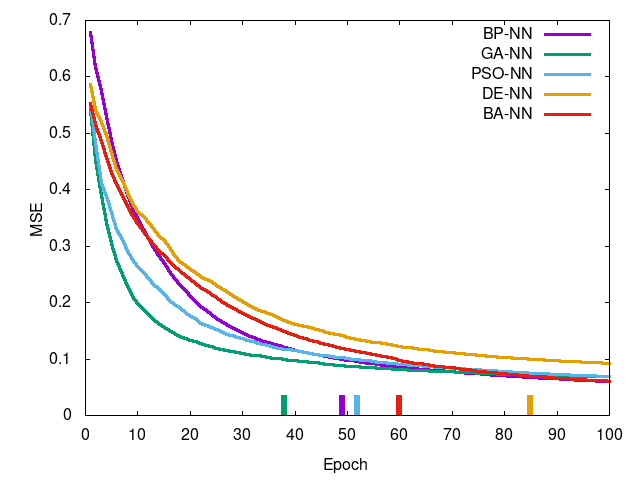
\includegraphics[scale=0.65]{images/wheat-plot.png}
\caption{Wheat Seeds test results for metaheuristics and backpropagation.}
\label{fig:wheat}
\end{figure}

To discover whether the curves are different to any meaningful degree, an ANOVA test is performed. This test yields an $F = 5.847$ with a $p < 0.001$, showing confidence that there is strong stochastic dominance between one or more samples.

Using Tukey's HSD test, each sample is examined and it is found that all samples---except DE-NN---come from the same distribution. This suggests there is no meaningful difference in choosing BP-NN, GA-NN, PSO-NN, or BP-NN. The only outlier is DE-NN.

While the ANOVA test showed significance, the significance is removed were DE-NN not a candidate sample for the tests, as pairwise difference of means between the other samples is insignificant.

\begin{table}[h!]
\centering
\begin{tabular}{c|c|c|c|c|c|}
\cline{2-6}
 & \textbf{BP-NN} & \textbf{GA-NN} & \textbf{PSO-NN} & \textbf{DE-NN} & \textbf{BA-NN} \\ \hline
\multicolumn{1}{|c|}{\textit{Min}} & \cellcolor[HTML]{FFFFFF}29 & \cellcolor[HTML]{C5F1BF}15 & \cellcolor[HTML]{FFFFFF}16 & \cellcolor[HTML]{FFCCC9}53 & \cellcolor[HTML]{FFFFFF}27 \\ \hline
\multicolumn{1}{|c|}{\textit{Avg}} & \cellcolor[HTML]{FFFFFF}49 & \cellcolor[HTML]{C5F1BF}38 & \cellcolor[HTML]{FFFFFF}52 & \cellcolor[HTML]{FFCCC9}85 & \cellcolor[HTML]{FFFFFF}60 \\ \hline
\end{tabular}
\caption{Minimum and average time to terminate for Wheat Seeds data set.}
\label{Tab:wheat-min}
\end{table}

Upon looking at the table above, this is the first test where GA-NN was fastest to converge in single-run training and on average. For the smaller problems, GA-NN was best in one or the other but it is interesting to see it outperform all other methods tested. However, since there is no significance in choosing it over the others, these results are inconclusive.

\pagebreak

\subsection{Wine}

The Wine data set is trained upon using the previously defined network parameters. The below plot is made using those results:

\begin{figure}[h!]
\centering
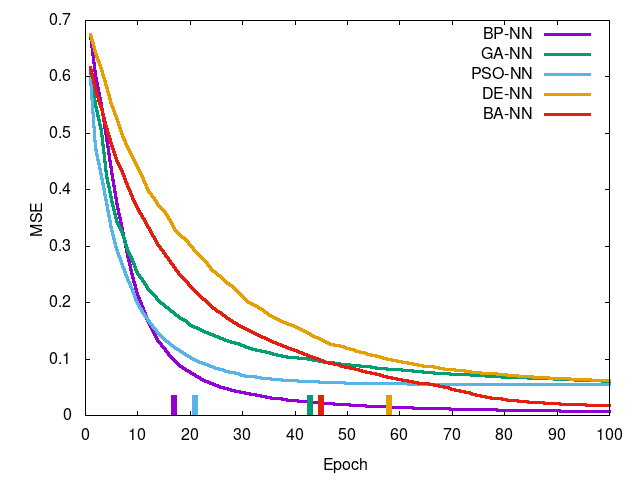
\includegraphics[scale=0.65]{images/wine-plot.png}
\caption{Wine test results for metaheuristics and backpropagation.}
\label{fig:wine}
\end{figure}

It is hard to determine which samples come from the same distribution, so an ANOVA test is performed yielding an $F = 12.081$, suggesting strong confidence in the test, and a $p < 0.001$ meaning strong significance in choosing some training methods over others.

To determine this, Tukey's HSD test is performed and the results are examined. The test suggests the curves come from three distributions: BP-NN and PSO-NN belong to the same distribution with strong confidence; GA-NN and BA-NN likewise belong to the same distribution; DE-NN is an outlier to each.

From this test, it can be surmised there is strong favor to choosing BP-NN or PSO-NN over other training methods.

\begin{table}[h!]
\centering
\begin{tabular}{c|c|c|c|c|c|}
\cline{2-6}
 & \textbf{BP-NN} & \textbf{GA-NN} & \textbf{PSO-NN} & \textbf{DE-NN} & \textbf{BA-NN} \\ \hline
\multicolumn{1}{|c|}{\textit{Min}} & \cellcolor[HTML]{FFFFFF}14 & \cellcolor[HTML]{FFFFFF}19 & \cellcolor[HTML]{C5F1BF}13 & \cellcolor[HTML]{FFCCC9}37 & \cellcolor[HTML]{FFFFFF}19 \\ \hline
\multicolumn{1}{|c|}{\textit{Avg}} & \cellcolor[HTML]{C5F1BF}17 & \cellcolor[HTML]{FFFFFF}43 & \cellcolor[HTML]{FFFFFF}21 & \cellcolor[HTML]{FFCCC9}58 & \cellcolor[HTML]{FFFFFF}45 \\ \hline
\end{tabular}
\caption{Minimum and average time to terminate for Wine data set.}
\label{Tab:wine-min}
\end{table}

As before, a table is generated of the minimum and average number of epochs it took for each training method to converge.

Since BP-NN and PSO-NN have the smallest mean and minimum number of epochs to converge and they belong to the same distribution, either training method is preferable to the others. Of methods to choose, however, DE-NN is the outlier with the worst performance.

Interestingly, up to this point, GA-NN has been fastest to converge in single runs, on average, or both. This is the first problem where it is neither.

\pagebreak

\subsection{Breast Cancer}

The Breast Cancer data set is then trained upon which yields the below plot using the defined network parameters for each training method:

\begin{figure}[h!]
\centering
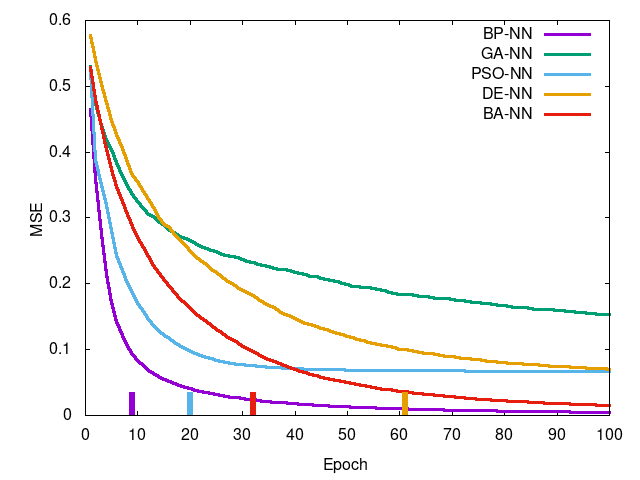
\includegraphics[scale=0.65]{images/breast-plot.png}
\caption{Breast Cancer test results for metaheuristics and backpropagation.}
\label{fig:breast}
\end{figure}

As with the Penguins data set, it is difficult to discern how related or unrelated each curve is other than GA-NN not converging.

To understand the plot better, an ANOVA test is performed yielding an $F=61.494$ and $p < 0.001$ suggesting strong significance in choosing one or some training methods over others.

Tukey's HSD test is again performed to determine which samples come from the same distribution. The test reveals strong favor in choosing BP-NN over other methods. There is no significance in choosing PSO-NN over BA-NN or vice-versa, but there is slight significance in choosing BP-NN other either.

\begin{table}[h!]
\centering
\begin{tabular}{c|c|c|c|c|c|}
\cline{2-6}
 & \textbf{BP-NN} & \textbf{GA-NN} & \textbf{PSO-NN} & \textbf{DE-NN} & \textbf{BA-NN} \\ \hline
\multicolumn{1}{|c|}{\textit{Min}} & \cellcolor[HTML]{C5F1BF}6 & \cellcolor[HTML]{FFCCC9}52 & 11 & 37 & 16 \\ \hline
\multicolumn{1}{|c|}{\textit{Avg}} & \cellcolor[HTML]{C5F1BF}9 & \cellcolor[HTML]{FFCCC9}DNC & 20 & 61 & 32 \\ \hline
\end{tabular}
\caption{Minimum and average time to terminate for Breast Cancer set.}
\label{Tab:breast-min}
\end{table}

In the table above, performance is measured for each training method by way of the mean and minimum amount of epochs to reach termination condition. A "DNC" here, under GA-NN, means the training method did not converge.

As suggested by Tukey's HSD test, BP-NN has the speed advantage over the other training methods for the Breast Cancer classification problem.

\pagebreak

\subsection{Ionosphere Radar}

The final data set, Ionosphere Radar, is test and plotted according to the previously defined network parameters:

\begin{figure}[h!]
\centering
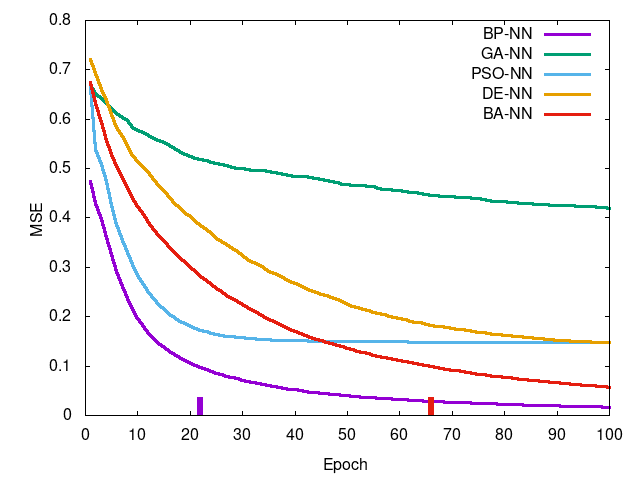
\includegraphics[scale=0.65]{images/ionosphere-plot.png}
\caption{Ionosphere Radar test results for metaheuristics and backpropagation.}
\label{fig:ionosphere}
\end{figure}

Here, only two training techniques converged within the allotted number of training iterations: BP-NN and BA-NN. 

Visually, it is clear there is difference to the two methods, but to verify, an ANOVA test is performed, producing an $F = 185.7$, a very high $F$-score, and a $p < 0.001$, concluding that there is a large degree of significance between BP-NN and BA-NN.

Tukey's HSD test shows pairwise significance between samples as significant for all samples. What can be deduced from this is that between the two methods that converged, BP-NN is considerably faster.

\begin{table}[h!]
\centering
\begin{tabular}{c|c|c|c|c|c|}
\cline{2-6}
 & \textbf{BP-NN} & \textbf{GA-NN} & \textbf{PSO-NN} & \textbf{DE-NN} & \textbf{BA-NN} \\ \hline
\multicolumn{1}{|c|}{\textit{Min}} & \cellcolor[HTML]{C5F1BF}9 & \cellcolor[HTML]{FFCCC9}DNC & 24 & 84 & 23 \\ \hline
\multicolumn{1}{|c|}{\textit{Avg}} & \cellcolor[HTML]{C5F1BF}22 & \cellcolor[HTML]{FFCCC9}DNC & \cellcolor[HTML]{FFCCC9}DNC & \cellcolor[HTML]{FFCCC9}DNC & 66 \\ \hline
\end{tabular}
\caption{Minimum and average time to terminate for Ionosphere Radar set.}
\label{Tab:ionosphere-min}
\end{table}

Finally, a table is constructed showing the minimum and average number of epochs to reach a termination condition. As before, a "DNC" signifies the training method did not converge.

While PSO-NN and DE-NN could converge, on average they were unable to. Notable is GA-NN was unable to converge during any training runs. As alluded to from the ANOVA and Tukey HSD tests, BP-NN is the fastest training method for this problem.

\pagebreak

\section{Results Summary}

\section{Conclusion}

\bibliographystyle{abbrv}
\bibliography{references}

\end{document}